%!TEX root = egpaper_for_review.tex
\begin{figure*}
\tikzstyle{cedge}=[fill=white,dotted,font=\sffamily\tiny, opacity=0.5, text=gray]
\tikzstyle{aedge}=[fill=white,solid,font=\sffamily\tiny, text=black!70          ]
\tikzstyle{vert}=[circle,minimum size = 0.5cm,inner sep = 1pt,draw, font=\small,align=left]
\centering
\begin{subfigure}[t]{0.20\linewidth}
   %\begin{framed}
   \resizebox{1.0\linewidth}{!}{
      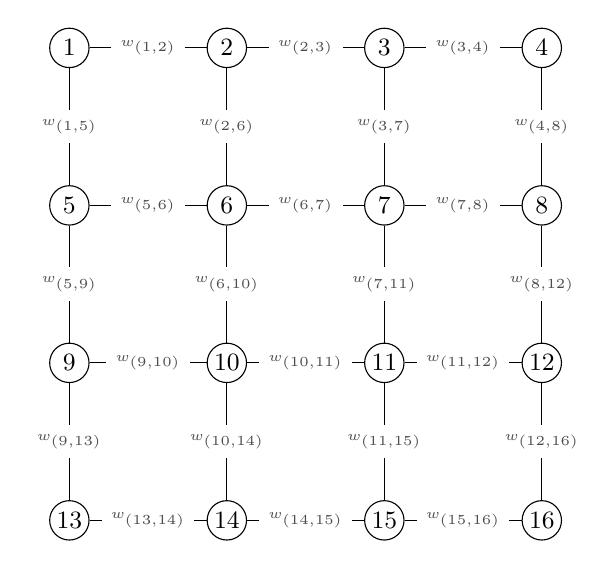
\begin{tikzpicture}[scale=1.0,transform shape]
        \tikzstyle{vert}=[circle,minimum size = 0.5cm,inner sep = 0pt,draw, font=\small, node distance = 5cm]
        \draw (0*2,3*2) node[vert](1){$1$};
        \draw (1*2,3*2) node[vert](2){$2$};
        \draw (2*2,3*2) node[vert](3){$3$};
        \draw (3*2,3*2) node[vert](4){$4$};
        \draw (0*2,2*2) node[vert](5){$5$};
        \draw (1*2,2*2) node[vert](6){$6$};
        \draw (2*2,2*2) node[vert](7){$7$};
        \draw (3*2,2*2) node[vert](8){$8$};
        \draw (0*2,1*2) node[vert](9){$9$};
        \draw (1*2,1*2) node[vert](10){$10$};
        \draw (2*2,1*2) node[vert](11){$11$};
        \draw (3*2,1*2) node[vert](12){$12$};
        \draw (0*2,0*2) node[vert](13){$13$};
        \draw (1*2,0*2) node[vert](14){$14$};
        \draw (2*2,0*2) node[vert](15){$15$};
        \draw (3*2,0*2) node[vert](16){$16$};
        %
        \path[every node/.style={font=\sffamily\tiny, fill=white}]
            (1)     edge[aedge]     node{$w_{(1, 2)}$   }     (2)
            (2)     edge[aedge]     node{$w_{(2, 3)}$   }     (3)
            (3)     edge[aedge]     node{$w_{(3, 4)}$   }     (4)
            (5)     edge[aedge]     node{$w_{(5, 6)}$   }     (6)
            (6)     edge[aedge]     node{$w_{(6, 7)}$   }     (7)
            (7)     edge[aedge]     node{$w_{(7, 8)}$   }     (8)
            (9)     edge[aedge]     node{$w_{(9, 10)}$  }     (10)
            (10)    edge[aedge]     node{$w_{(10, 11)}$ }     (11)
            (11)    edge[aedge]     node{$w_{(11, 12)}$ }     (12)
            (13)    edge[aedge]     node{$w_{(13, 14)}$ }     (14)
            (14)    edge[aedge]     node{$w_{(14, 15)}$ }     (15)
            (15)    edge[aedge]     node{$w_{(15, 16)}$ }     (16)
            (1)     edge[aedge]     node{$w_{(1, 5)}$   }     (5)
            (5)     edge[aedge]     node{$w_{(5, 9)}$   }     (9)
            (9)     edge[aedge]     node{$w_{(9, 13)}$  }     (13)
            (2)     edge[aedge]     node{$w_{(2, 6)}$   }     (6)
            (6)     edge[aedge]     node{$w_{(6, 10)}$  }     (10)
            (10)    edge[aedge]     node{$w_{(10, 14)}$ }     (14)
            (3)     edge[aedge]     node{$w_{(3, 7)}$   }     (7)
            (7)     edge[aedge]     node{$w_{(7, 11)}$  }     (11)
            (11)    edge[aedge]     node{$w_{(11, 15)}$ }     (15)
            (4)     edge[aedge]     node{$w_{(4, 8)}$   }     (8)
            (8)     edge[aedge]     node{$w_{(8, 12)}$  }     (12)
            (12)    edge[aedge]     node{$w_{(12, 16)}$ }     (16)
        ;
      \end{tikzpicture}
   }
   %\end{framed} 
\caption{Graph $\mathcal{G}$}    
\end{subfigure}\quad\quad
\begin{subfigure}[t]{0.20\linewidth}
   %\begin{framed}
   \resizebox{1.0\linewidth}{!}{
      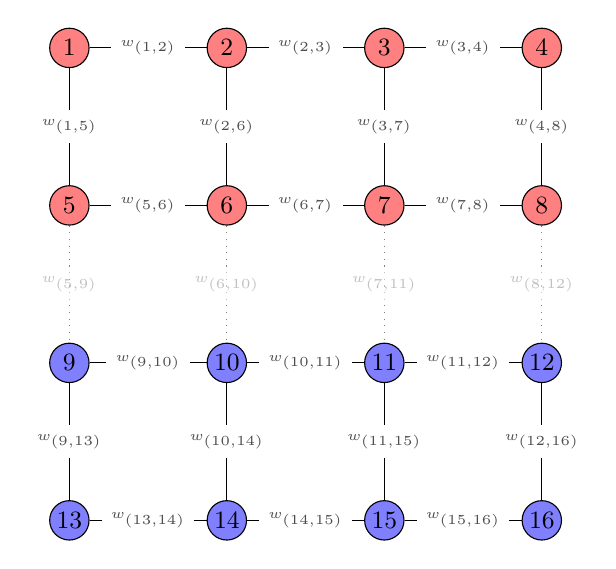
\begin{tikzpicture}[scale=1.0,transform shape]

        \draw (0*2,3*2) node[vert,fill=red!50](1){$1$};
        \draw (1*2,3*2) node[vert,fill=red!50](2){$2$};
        \draw (2*2,3*2) node[vert,fill=red!50](3){$3$};
        \draw (3*2,3*2) node[vert,fill=red!50](4){$4$};
        \draw (0*2,2*2) node[vert,fill=red!50](5){$5$};
        \draw (1*2,2*2) node[vert,fill=red!50](6){$6$};
        \draw (2*2,2*2) node[vert,fill=red!50](7){$7$};
        \draw (3*2,2*2) node[vert,fill=red!50](8){$8$};
        \draw (0*2,1*2) node[vert,fill=blue!50](9){$9$};
        \draw (1*2,1*2) node[vert,fill=blue!50](10){$10$};
        \draw (2*2,1*2) node[vert,fill=blue!50](11){$11$};
        \draw (3*2,1*2) node[vert,fill=blue!50](12){$12$};
        \draw (0*2,0*2) node[vert,fill=blue!50](13){$13$};
        \draw (1*2,0*2) node[vert,fill=blue!50](14){$14$};
        \draw (2*2,0*2) node[vert,fill=blue!50](15){$15$};
        \draw (3*2,0*2) node[vert,fill=blue!50](16){$16$};
        %
        \path[every node/.style={font=\sffamily\tiny, fill=white}]
            (1)     edge[aedge]     node{$w_{(1, 2)}$   }     (2)
            (2)     edge[aedge]     node{$w_{(2, 3)}$   }     (3)
            (3)     edge[aedge]     node{$w_{(3, 4)}$   }     (4)
            (5)     edge[aedge]     node{$w_{(5, 6)}$   }     (6)
            (6)     edge[aedge]     node{$w_{(6, 7)}$   }     (7)
            (7)     edge[aedge]     node{$w_{(7, 8)}$   }     (8)
            (9)     edge[aedge]     node{$w_{(9, 10)}$  }     (10)
            (10)    edge[aedge]     node{$w_{(10, 11)}$ }     (11)
            (11)    edge[aedge]     node{$w_{(11, 12)}$ }     (12)
            (13)    edge[aedge]     node{$w_{(13, 14)}$ }     (14)
            (14)    edge[aedge]     node{$w_{(14, 15)}$ }     (15)
            (15)    edge[aedge]     node{$w_{(15, 16)}$ }     (16)
            (1)     edge[aedge]     node{$w_{(1, 5)}$   }     (5)
            (5)     edge[cedge]     node{$w_{(5, 9)}$   }     (9)
            (9)     edge[aedge]     node{$w_{(9, 13)}$  }     (13)
            (2)     edge[aedge]     node{$w_{(2, 6)}$   }     (6)
            (6)     edge[cedge]     node{$w_{(6, 10)}$  }     (10)
            (10)    edge[aedge]     node{$w_{(10, 14)}$ }     (14)
            (3)     edge[aedge]     node{$w_{(3, 7)}$   }     (7)
            (7)     edge[cedge]     node{$w_{(7, 11)}$  }     (11)
            (11)    edge[aedge]     node{$w_{(11, 15)}$ }     (15)
            (4)     edge[aedge]     node{$w_{(4, 8)}$   }     (8)
            (8)     edge[cedge]     node{$w_{(8, 12)}$  }     (12)
            (12)    edge[aedge]     node{$w_{(12, 16)}$ }     (16)
        ;
      \end{tikzpicture}
   }
   %\end{framed}
\caption{$\mathcal{E}^A_{cut}$}
\end{subfigure}\quad\quad
\begin{subfigure}[t]{0.20\linewidth}
   %\begin{framed}
   \resizebox{1.0\linewidth}{!}{
      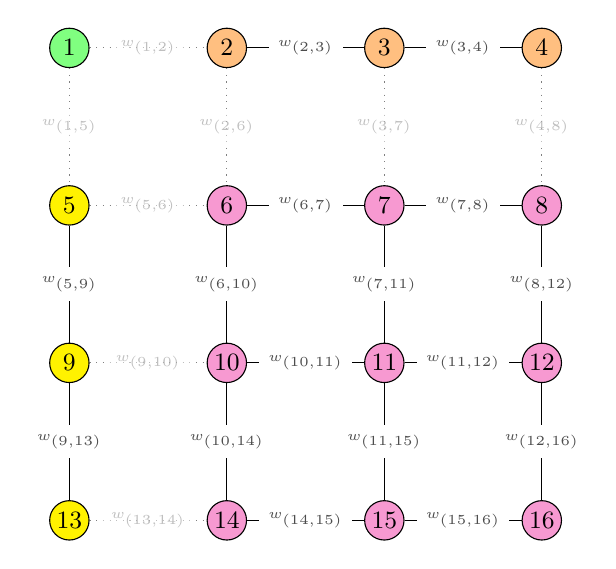
\begin{tikzpicture}[scale=1.0,transform shape]

        \draw (0*2,3*2) node[vert,fill=green!50](1){$1$};
        \draw (1*2,3*2) node[vert,fill=orange!50](2){$2$};
        \draw (2*2,3*2) node[vert,fill=orange!50](3){$3$};
        \draw (3*2,3*2) node[vert,fill=orange!50](4){$4$};
        \draw (0*2,2*2) node[vert,fill=yellow!=30](5){$5$};
        \draw (1*2,2*2) node[vert,fill=magenta!40](6){$6$};
        \draw (2*2,2*2) node[vert,fill=magenta!40](7){$7$};
        \draw (3*2,2*2) node[vert,fill=magenta!40](8){$8$};
        \draw (0*2,1*2) node[vert,fill=yellow!=30](9){$9$};
        \draw (1*2,1*2) node[vert,fill=magenta!40](10){$10$};
        \draw (2*2,1*2) node[vert,fill=magenta!40](11){$11$};
        \draw (3*2,1*2) node[vert,fill=magenta!40](12){$12$};
        \draw (0*2,0*2) node[vert,fill=yellow!=30](13){$13$};
        \draw (1*2,0*2) node[vert,fill=magenta!40](14){$14$};
        \draw (2*2,0*2) node[vert,fill=magenta!40](15){$15$};
        \draw (3*2,0*2) node[vert,fill=magenta!40](16){$16$};
        %
        \path[every node/.style={font=\sffamily\tiny, fill=white}]
            (1)     edge[cedge]     node{$w_{(1, 2)}$   }     (2)
            (2)     edge[aedge]     node{$w_{(2, 3)}$   }     (3)
            (3)     edge[aedge]     node{$w_{(3, 4)}$   }     (4)
            (5)     edge[cedge]     node{$w_{(5, 6)}$   }     (6)
            (6)     edge[aedge]     node{$w_{(6, 7)}$   }     (7)
            (7)     edge[aedge]     node{$w_{(7, 8)}$   }     (8)
            (9)     edge[cedge]     node{$w_{(9, 10)}$  }     (10)
            (10)    edge[aedge]     node{$w_{(10, 11)}$ }     (11)
            (11)    edge[aedge]     node{$w_{(11, 12)}$ }     (12)
            (13)    edge[cedge]     node{$w_{(13, 14)}$ }     (14)
            (14)    edge[aedge]     node{$w_{(14, 15)}$ }     (15)
            (15)    edge[aedge]     node{$w_{(15, 16)}$ }     (16)
            (1)     edge[cedge]     node{$w_{(1, 5)}$   }     (5)
            (5)     edge[aedge]     node{$w_{(5, 9)}$   }     (9)
            (9)     edge[aedge]     node{$w_{(9, 13)}$  }     (13)
            (2)     edge[cedge]     node{$w_{(2, 6)}$   }     (6)
            (6)     edge[aedge]     node{$w_{(6, 10)}$  }     (10)
            (10)    edge[aedge]     node{$w_{(10, 14)}$ }     (14)
            (3)     edge[cedge]     node{$w_{(3, 7)}$   }     (7)
            (7)     edge[aedge]     node{$w_{(7, 11)}$  }     (11)
            (11)    edge[aedge]     node{$w_{(11, 15)}$ }     (15)
            (4)     edge[cedge]     node{$w_{(4, 8)}$   }     (8)
            (8)     edge[aedge]     node{$w_{(8, 12)}$  }     (12)
            (12)    edge[aedge]     node{$w_{(12, 16)}$ }     (16)
        ;
      \end{tikzpicture}
   }
   %\end{framed}
\caption{$\mathcal{E}^B_{cut}$}  
\end{subfigure}\quad\quad
\begin{subfigure}[t]{0.20\linewidth}
   %\begin{framed}
   \resizebox{1.0\linewidth}{!}{
      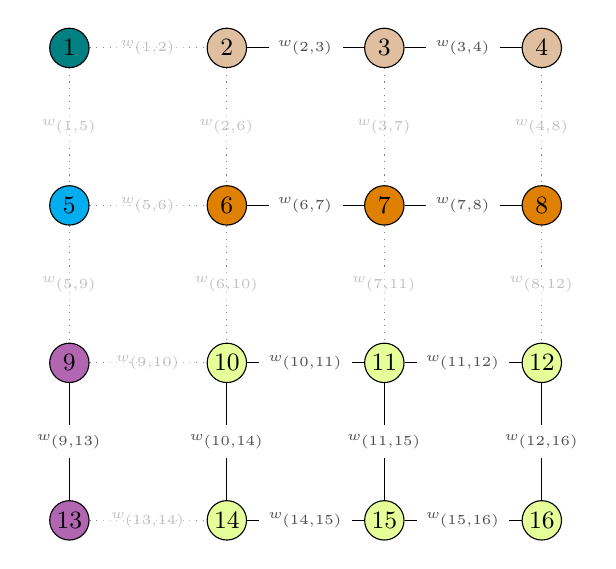
\begin{tikzpicture}[scale=1.0,transform shape]

        \draw (0*2,3*2) node[vert,fill=blue!50!green](1){$1$};
        \draw (1*2,3*2) node[vert,fill=brown!50](2){$2$};
        \draw (2*2,3*2) node[vert,fill=brown!50](3){$3$};
        \draw (3*2,3*2) node[vert,fill=brown!50](4){$4$};
        \draw (0*2,2*2) node[vert,fill=cyan!=30](5){$5$};
        \draw (1*2,2*2) node[vert,fill=red!50!lime](6){$6$};
        \draw (2*2,2*2) node[vert,fill=red!50!lime](7){$7$};
        \draw (3*2,2*2) node[vert,fill=red!50!lime](8){$8$};
        \draw (0*2,1*2) node[vert,fill=violet!60](9){$9$};
        \draw (1*2,1*2) node[vert,fill=lime!40](10){$10$};
        \draw (2*2,1*2) node[vert,fill=lime!40](11){$11$};
        \draw (3*2,1*2) node[vert,fill=lime!40](12){$12$};
        \draw (0*2,0*2) node[vert,fill=violet!60](13){$13$};
        \draw (1*2,0*2) node[vert,fill=lime!40](14){$14$};
        \draw (2*2,0*2) node[vert,fill=lime!40](15){$15$};
        \draw (3*2,0*2) node[vert,fill=lime!40](16){$16$};
        %
        \path[every node/.style={font=\sffamily\tiny, fill=white}]
            (1)     edge[cedge]     node{$w_{(1, 2)}$   }     (2)
            (2)     edge[aedge]     node{$w_{(2, 3)}$   }     (3)
            (3)     edge[aedge]     node{$w_{(3, 4)}$   }     (4)
            (5)     edge[cedge]     node{$w_{(5, 6)}$   }     (6)
            (6)     edge[aedge]     node{$w_{(6, 7)}$   }     (7)
            (7)     edge[aedge]     node{$w_{(7, 8)}$   }     (8)
            (9)     edge[cedge]     node{$w_{(9, 10)}$  }     (10)
            (10)    edge[aedge]     node{$w_{(10, 11)}$ }     (11)
            (11)    edge[aedge]     node{$w_{(11, 12)}$ }     (12)
            (13)    edge[cedge]     node{$w_{(13, 14)}$ }     (14)
            (14)    edge[aedge]     node{$w_{(14, 15)}$ }     (15)
            (15)    edge[aedge]     node{$w_{(15, 16)}$ }     (16)
            (1)     edge[cedge]     node{$w_{(1, 5)}$   }     (5)
            (5)     edge[cedge]     node{$w_{(5, 9)}$   }     (9)
            (9)     edge[aedge]     node{$w_{(9, 13)}$  }     (13)
            (2)     edge[cedge]     node{$w_{(2, 6)}$   }     (6)
            (6)     edge[cedge]     node{$w_{(6, 10)}$  }     (10)
            (10)    edge[aedge]     node{$w_{(10, 14)}$ }     (14)
            (3)     edge[cedge]     node{$w_{(3, 7)}$   }     (7)
            (7)     edge[cedge]     node{$w_{(7, 11)}$  }     (11)
            (11)    edge[aedge]     node{$w_{(11, 15)}$ }     (15)
            (4)     edge[cedge]     node{$w_{(4, 8)}$   }     (8)
            (8)     edge[cedge]     node{$w_{(8, 12)}$  }     (12)
            (12)    edge[aedge]     node{$w_{(12, 16)}$ }     (16)
        ;
      \end{tikzpicture}
   }
   %\end{framed}
\caption{$\mathcal{E}^{AB}_{cut} = \mathcal{E}^B_{cut} \cup \mathcal{E}^B_{cut}$}  
\end{subfigure}

\vspace{0.1cm}

\begin{subfigure}[t]{0.20\linewidth}
   %\begin{framed}
   \resizebox{1.0\linewidth}{!}{
      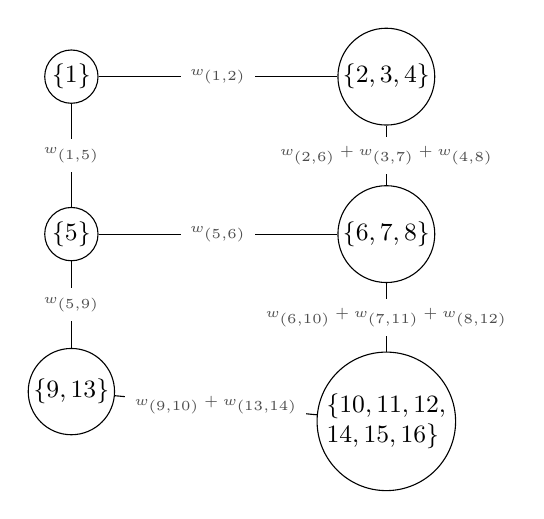
\begin{tikzpicture}[scale=1.0,transform shape]
        \draw (0*2,3*2) node[vert](1){$\{1\}$};
        \draw (2*2,3*2) node[vert](2){$\{2, 3, 4\}$};
        \draw (0*2,2*2) node[vert,](5){$\{5\}$};
        \draw (2*2,2*2) node[vert](6){$\{6, 7, 8\}$};
        \draw (0*2,1*2) node[vert](9){$\{9, 13\}$};
        \draw (2*2,0.811*2) node[vert ](10){$\{10, 11, 12,$\\$14, 15, 16\}$};
        %
        \path[every node/.style={font=\sffamily\tiny, fill=white}]
            (1)     edge[aedge]     node{$w_{(1, 2)}$   }     (2)
            (1)     edge[aedge]     node{$w_{(1, 5)}$   }     (5)
            (1)     edge[aedge]     node{$w_{(1, 5)}$   }     (5)
            (5)     edge[aedge]     node{$w_{(5, 6)}$   }     (6)
            (5)     edge[aedge]     node{$w_{(5, 9)}$   }     (9)
            (9)     edge[aedge]     node{$w_{(9, 10)} + w_{(13, 14)}$   }     (10)
            (2)     edge[aedge]     node{$w_{(2, 6)} + w_{(3, 7)} + w_{(4, 8)} $   }     (6)
            (6)     edge[aedge]     node{$w_{(6, 10)} + w_{(7, 11)} + w_{(8, 12)} $   }     (10)
        ;
        %;
      \end{tikzpicture}
   }
   %\end{framed}
\caption{$\mathcal{\bar{G}}=\textbf{\scriptsize{contract}}(\mathcal{E} \backslash \{\mathcal{E}^{AB}_{cut}\})$}
\end{subfigure}
\quad\quad\quad
\begin{subfigure}[t]{0.20\linewidth}
   %\begin{framed}
   \resizebox{1.0\linewidth}{!}{
      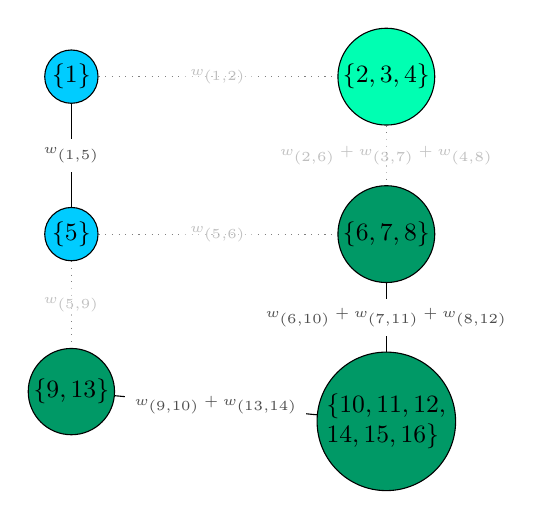
\begin{tikzpicture}[scale=1.0,transform shape]
        \draw (0*2,3*2) node[vert,fill=blue!20!cyan](1){$\{1\}$};
        \draw (2*2,3*2) node[vert,fill=green!30!cyan](2){$\{2, 3, 4\}$};
        \draw (0*2,2*2) node[vert,fill=blue!20!cyan ](5){$\{5\}$};
        \draw (2*2,2*2) node[vert,fill=blue!40!green](6){$\{6, 7, 8\}$};
        \draw (0*2,1*2) node[vert,fill=blue!40!green](9){$\{9, 13\}$};
        \draw (2*2,0.811*2) node[vert,fill=blue!40!green](10){$\{10, 11, 12,$\\$14, 15, 16\}$};
        %
        \path[every node/.style={font=\sffamily\tiny, fill=white}]
            (1)     edge[cedge]     node{$w_{(1, 2)}$   }     (2)
            (1)     edge[cedge]     node{$w_{(1, 5)}$   }     (5)
            (1)     edge[aedge]     node{$w_{(1, 5)}$   }     (5)
            (5)     edge[cedge]     node{$w_{(5, 6)}$   }     (6)
            (5)     edge[cedge]     node{$w_{(5, 9)}$   }     (9)
            (9)     edge[aedge]     node{$w_{(9, 10)} + w_{(13, 14)}$   }     (10)
            (2)     edge[cedge]     node{$w_{(2, 6)} + w_{(3, 7)} + w_{(4, 8)} $   }     (6)
            (6)     edge[aedge]     node{$w_{(6, 10)} + w_{(7, 11)} + w_{(8, 12)} $   }     (10)
        ;
        %;
      \end{tikzpicture}
   }
   %\end{framed}
\caption{$\mathcal{E}_{\textit{\tiny{cut}}}^{\bar{\mathcal{G}}}  $}
\end{subfigure}
\quad\quad\quad
\begin{subfigure}[t]{0.20\linewidth}
   %\begin{framed}
   \resizebox{1.0\linewidth}{!}{
      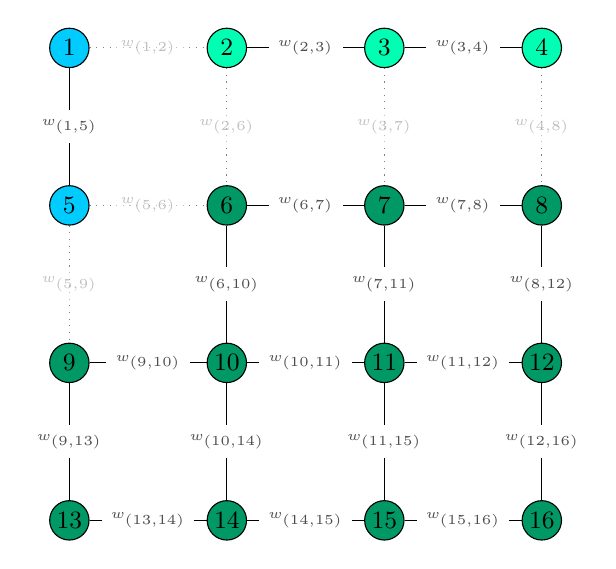
\begin{tikzpicture}[scale=1.0,transform shape]

        \draw (0*2,3*2) node[vert,fill=blue!20!cyan](1){$1$};
        \draw (1*2,3*2) node[vert,fill=green!30!cyan](2){$2$};
        \draw (2*2,3*2) node[vert,fill=green!30!cyan](3){$3$};
        \draw (3*2,3*2) node[vert,fill=green!30!cyan](4){$4$};
        \draw (0*2,2*2) node[vert,fill=blue!20!cyan](5){$5$};
        \draw (1*2,2*2) node[vert,fill=blue!40!green](6){$6$};
        \draw (2*2,2*2) node[vert,fill=blue!40!green](7){$7$};
        \draw (3*2,2*2) node[vert,fill=blue!40!green](8){$8$};
        \draw (0*2,1*2) node[vert,fill=blue!40!green](9){$9$};
        \draw (1*2,1*2) node[vert,fill=blue!40!green](10){$10$};
        \draw (2*2,1*2) node[vert,fill=blue!40!green](11){$11$};
        \draw (3*2,1*2) node[vert,fill=blue!40!green](12){$12$};
        \draw (0*2,0*2) node[vert,fill=blue!40!green](13){$13$};
        \draw (1*2,0*2) node[vert,fill=blue!40!green](14){$14$};
        \draw (2*2,0*2) node[vert,fill=blue!40!green](15){$15$};
        \draw (3*2,0*2) node[vert,fill=blue!40!green](16){$16$};
        %
        \path[every node/.style={font=\sffamily\tiny, fill=white}]
            (1)     edge[cedge]     node{$w_{(1, 2)}$   }     (2)
            (2)     edge[aedge]     node{$w_{(2, 3)}$   }     (3)
            (3)     edge[aedge]     node{$w_{(3, 4)}$   }     (4)
            (5)     edge[cedge]     node{$w_{(5, 6)}$   }     (6)
            (6)     edge[aedge]     node{$w_{(6, 7)}$   }     (7)
            (7)     edge[aedge]     node{$w_{(7, 8)}$   }     (8)
            (9)     edge[aedge]     node{$w_{(9, 10)}$  }     (10)
            (10)    edge[aedge]     node{$w_{(10, 11)}$ }     (11)
            (11)    edge[aedge]     node{$w_{(11, 12)}$ }     (12)
            (13)    edge[aedge]     node{$w_{(13, 14)}$ }     (14)
            (14)    edge[aedge]     node{$w_{(14, 15)}$ }     (15)
            (15)    edge[aedge]     node{$w_{(15, 16)}$ }     (16)
            (1)     edge[aedge]     node{$w_{(1, 5)}$   }     (5)
            (5)     edge[cedge]     node{$w_{(5, 9)}$   }     (9)
            (9)     edge[aedge]     node{$w_{(9, 13)}$  }     (13)
            (2)     edge[cedge]     node{$w_{(2, 6)}$   }     (6)
            (6)     edge[aedge]     node{$w_{(6, 10)}$  }     (10)
            (10)    edge[aedge]     node{$w_{(10, 14)}$ }     (14)
            (3)     edge[cedge]     node{$w_{(3, 7)}$   }     (7)
            (7)     edge[aedge]     node{$w_{(7, 11)}$  }     (11)
            (11)    edge[aedge]     node{$w_{(11, 15)}$ }     (15)
            (4)     edge[cedge]     node{$w_{(4, 8)}$   }     (8)
            (8)     edge[aedge]     node{$w_{(8, 12)}$  }     (12)
            (12)    edge[aedge]     node{$w_{(12, 16)}$ }     (16)
        ;
      \end{tikzpicture}
   }
   %\end{framed}
\caption{$\mathcal{E}_{\textit{\tiny{cut}}}^{\bar{\mathcal{G}}}=\textbf{\scriptsize{projectBack}} (\mathcal{E}_{\textit{\tiny{cut}}}^{\bar{\mathcal{G}}} )  $}
\end{subfigure}
\caption{
        Describe Method here
}
\end{figure*}
